\chapter{Experiments and Results} %experimental results
We set up our system  on ``Saguaro'' one of the three computing environments provided by ASU for research purposes. Saguaro is a 5K processor Dell Linux cluster which can perform almost 45 million floating point operation per second, it has over 9 Tera bytes of RAM and over 400 Terra Bytes aggregate disk space. A node on Saguaro can be easily and conveniently accessed via a SSH protocol. Each node has 8 processors and 16GB of RAM. I acquired a node on saguaro during the summer of 2015.

\section{Experimental Setup}
In prior work ~\cite{zhang2016applying} the authors study the surface deformation of the hippocampal region of the brain and use it as features for training a dictionary of basis vectors and associated sparse codes. This encoding learn sets of over complete basis vectors which are better able to capture structures and patterns inherent in the input data. The hippocampal surface is modeled from the hippocampal region of the brain and patches on its surface captures topological information effectively. Similar a system can be designed which uses a patch based feature extraction process and then use statistics derives form the patches for classification. However an important question for diagnostic classification based on voxel-based or surface-based maps is which statistics are best to analyze. 

\citep{kakimoto2011new} used the total z-score from the Brodmann Area sensitivity map in the brain surface, ~\citep{lu2017early} calculated the mean voxel values from 116 VOIs, standard deviations of voxel values from the 116 anatomical VOIs, and mean voxel value differences between 54 pairs of the anatomical VOIs on left and right brain hemispheres. All VOIs were extracted form a AAL template similar to the one in Fig.~\ref{fig:mask} with more regions of varying intensities. We hypothesize that a patch based extraction methods which selects overlapping volumes from each image in a number of samples and learns there sparse representations via a dictionary can then be used for classification Alg.~\ref{alg:pipeline1}. To compare this system we design one more system Alg.~\ref{alg:pipeline2} in which we directly pool intensities in the patch volume to a max. Maxing the overlapping patches ensure that the activation around a region is local to that volume. After which PCA can be applied to reduce the high dimension of the data and also helps in reducing noise induced for the blank patches (covering no region). We then evaluate the cerebral cortex as a potential imaging biomarker for AD diagnosis and prognosis research.  

The two systems we come up with are described below : 
\begin{enumerate}
	\item  Patch based Stochastic Coordinate Coding, Pooling the sparse codes to generate features for annotation, boosting features by adding gender, age, \apoe{1}, \apoe{2} and FAQ followed by classification. 
	\item Pooling $ n $ patches, using gender, age, \apoe{1}, \apoe{2} and FAQ as additional features for boosting classification, reducing the dimensions of the annotated patches and classification. 
\end{enumerate}

After normalizing, segmenting and skull stripping the cerebral cortex we extract features for classification.  In our experiments each processed FDG-PET is a $ 80 \times 95 \times 80 $ image with intensity values spread over the voxel volume. In this study we applied two different patch based extraction techniques. (1) For patch based sparse coding we compared 500, 1000 and 2000 number of patches to make the objective matrix for SCC. To reduce complexity we down sample 1000 dimensional patches to 125 dimensions by using a $ 2 \times 2 \times 2 $ window as described in Sec.~\ref{subsec:Patch_Generation_Dictionary_Learning}. (2) For patch based dimension reduction (PPCA) we made $ 4050 $ patches with varying overlap across the cerebral ROI-segmented FDG-PET volume. Fig.~\ref{fig:patches}(a,b) shows the patch formation for (1) and (2).

\begin{figure}
	\centering
	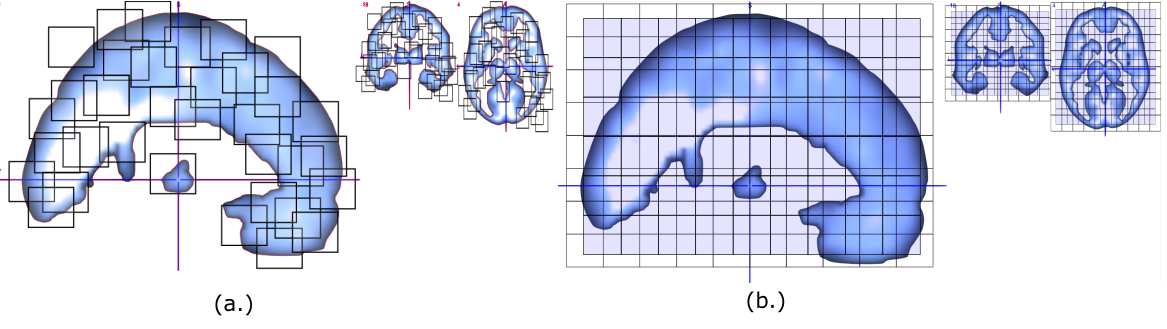
\includegraphics[width=\linewidth]{figures/patches}
	\caption[Unstructured and Structured patches in Axial, Sagittal and Coronal view of the brain.]{(a). Unstructured patches in Alg.1. The patches are generated randomly and ensure overlapping by creating enough of them. (b). Structured patches in Alg.2. with overlap shown in a slightly stronger shade of blue.}
	\label{fig:patches}
\end{figure}

In the training matrix we then involve additional features which enables us to make well defined classification, we include the genetic information and Functional Activities Questionnaire (FAQ) Scores even Age and Gender were involved. the two alleles of Apolipoprotein E(APOE) are available, APOE genotype is represented by combination of $e2$ (episilon 2),$e3$ and $e4$. Each individual will have one of the following combinations: $e2/e2$, $e2/e34$, $e2/e44$, $e3/e3$, $e3/e4$, $e4/e4$. Although the order between two genotypes for each person doesn't matter, they are represented in the order of $e2 \ge e3 \ge e4$. After feature annotation, the dimension of the dataset was reduced to a reasonable size and classification was performed.

\subsection{System Configuration}
We manage the data files on the cluster and use two system for the designing of both our systems. 

\begin{table}[h]
	\centering
	\begin{tabular}{|P{6cm}|P{7cm}|}
		\hline
		\multirow{4}*{Dell PowerEdge T110 II Server}
		& CPU : Intel Core2 Quad @ 2.6 GHz\\
		& OS : Windows 7\\
		&Total Memory (RAM) : 8 GB\\
		&No. of Cores : 4\\
		\midrule
		\multirow{4}*{Dell Alienware X1} 
		& CPU : Intel Core i5 @ 2.8 GHz\\
		& OS : Windows 10\\
		&Total Memory (RAM) : 16 GB\\ 
		&No. of Cores : 4\\
		\hline
	\end{tabular}
	\caption{System Configurations}
	\label{tab:system configurations}
\end{table}

\subsection{Languages and Software used.}
In this section we enumerate the software tools and languages used for the experiments.
\begin{enumerate}
\item Matlab (2016a,2015b) : To make the patches in both experiment \textbullet~ To max-pool the data in patch pooling and down-sampling the patches in (SCC) Section.~\ref{subsec:Patch_Generation_Dictionary_Learning}.  
\item C++ : To pool the learned dictionary \textbullet~ Sparse Coding, the code os taken from ~\citep{lin2014stochastic} and modified to fit our needs.
\item Python~(2.7.12) : For classification and file management
\item Shell : for scripting the above listed.
\item Software : SPM To preprocess the \FDGPET~ scans \textbullet~ InkScape for diagrams \textbullet~ Micron: for visualizing NiFTI files \textbullet ~MobaXterm / WinSCP / Putty: For accessing the cluster
\item Libraries : Python/2.7.12 (sklearn) for classifiers.
\end{enumerate}


 \section{Results}
\label{sec:Results}
We run six experiments over the two methods described in Algorithm~\ref{alg:pipeline1} (1) and Algorithm~\ref{alg:pipeline2} (2). An N-fold cross validation protocol was adopted to estimate classification accuracy. All subjects were randomly divided into N folds. The surface biomarkers were selected by training on N-1 folds and the test was performed on the remaining fold. We rotated this procedure for N times to estimate the accuracy. In this paper, we choose N = 10 to complete the classification.The output of each classification experiment was compared to the ground truth, and a contingency table was computed to indicate how many class labels were correctly identified as members of one of the two classes. The rows of the contingency table represent the true classes and the columns represent the assigned classes. The cell at row r and column $c$ is the number of subjects whose true class is r while their assigned class is $c$. Natural performance measures for classification problems mainly based on error rate or accuracy. However, higher accuracy does not necessarily imply better performance on target task. In two-category classification, one method for handling $c$-class problem is to consider $c$ 2-class problems: $ \frac{\omega_i}{not ~\omega_i} $~\citep{fawcett2004roc}. Therefore, confusion matrix was proposed as a method to measure classifier performance. TP, FP, TN, FN represents number of true positives, number of false positives, number of true negatives and number of false negative, respectively. The matrix in Table.~\ref{tab:confusion_matrix} represents a possible combination of ground truth and predicted classification for two classes.

\begin{table}[]
	\centering
	\begin{tabular}{|P{3.5cm}|P{3.5cm}|P{3.5cm}|}
		\hline
		& \multicolumn{2}{|P{7cm}|}{\emph{\bf Assigned Class}}\\
		\hline
		\emph{\bf True Class}& Positive & Negative \\
		\hline
		Positive & TP & FP \\
		Negative & FN & TN \\	
		\hline
	\end{tabular}
	\caption{The Confusion Matrix}
	\label{tab:confusion_matrix}
\end{table}

The total of TP, FP, FN, TN refers to the total number in the classification. Five performance measures \F~Score, Recall, Specificity, Positive predictive value and Negative predictive value were calculated as follows:

\begin{equation*}
\textrm{F}_1~\textrm{Score} = 2 \times \frac{\textrm{TP}}{\textrm{FN} + 2\times \textrm{TP} + \textrm{FP}}.
\end{equation*}

In a given population precision measures the amount of true cases classified correctly and recall the strength of that number. When you have both high precision and high recall it would mean that the population is well classified. \F~Score is the measure that is the harmonic mean of precision and recall. The reason for taking harmonic mean is because it is more appropriate when dealing rates and ratios.  

\begin{equation*}
\textrm{Recall} = \frac{\textrm{TP}}{\textrm{TP} + \textrm{FN}}.
\end{equation*}

Recall in this context is also referred as the true positive rate or sensitivity.  is a statistical measure of how well a binary classification test correctly identifies a condition and the probability of correctly labeling members of the target class.

\begin{equation*}
\textrm{Specificity} = \frac{\textrm{TN}}{\textrm{FP} + \textrm{TN}}.
\end{equation*}

The specificity is a statistical measure of how well a binary classification test correctly identifies the negative cases.

\begin{equation*}
\textrm{Positive predictive value} = \frac{\textrm{TP}}{\textrm{TP} + \textrm{FP}}.
\end{equation*}

Where positive predictive value (PPV) is also referred to as precision, which measures the probability of a positive prediction is correct.

\begin{equation*}
\textrm{Negative predictive value} = \frac{\textrm{TN}}{\textrm{TN} + \textrm{FN}}.
\end{equation*}

which measures the probability of a negative prediction is correct.

All these measures provide relevant information about the classification and no single measure tells the entire story. For example consider a scenario where 90\% of the population does not have a disease and the 10\% population is misclassified by the classifier, the accuracy would still be 90\%. Thus we should use multiple measures.   

There are some standard performance evaluation measures for classification study. Bigger values usually mean stronger classification power. We also computed the area-under-the-curve (AUC) of the receiver operating characteristic (ROC). The ROC is the average value of sensitivity for all the possible values of specificity. Such an index is especially useful in a comparative study of two diagnostic tests. If two tests are to be compared, it is desirable to compare the entire ROC curve rather than at a particular point~\citep{swets1979roc}. The maximum AUC=1 means that the diagnostic test is perfect in the differentiation between the diseased and stable. This happens when the distribution of test results for the diseased and stable do not overlap. AUC = 0.5 means the chance of discrimination that curve located on diagonal line in ROC space. Using these measures of analysis we first report the comparison between different sets of feature, followed by a thorough analysis on both the proposed pipelines. We then list the AUC comparison in the end.

\subsection{Comparison between Sets of Features.}
We tested our best scores across the features we have have in store for classification. In this comparison we put emphasis on the features we are including in classification. We tested both the pipelines using (1).Voxel information from the image (2). Voxels combined with rich genetic scores described in section.\ref{sec:Results} (3). A combination of (2) and the other demographic information. We observe that (3). gives very good results in AD vs. CU $ \sim 98\% $. Only in CU vs. LMCI (2) performs better with $ \sim 82 \% $    
\begin{table}[!h]
	\centering
	\begin{tabular}{P{3cm}P{3cm}P{2cm}P{3cm}P{3cm}}
		\hline
		Methods&Exp.& Voxels & Voxels + \apoe{2} + \apoe{3} + FAQ &  Voxels + \apoe{2} + \apoe{3} + FAQ + Age~\& Gender\\\hline
		\multirow{6}{*}{Pool+FE}
		& AD vs. CU		&$ 88.97 $&$ 95.10  $&$ 96.30 $\\
		& AD vs. EMCI 	&$ 76.92 $&$ 81.69 $&$ 83.68 $\\
		& AD vs. LMCI	&$ 63.26 $&$ 69.44 $&$ 73.42 $\\
		& CU vs. EMCI	&$ 54.49 $&$ 62.63 $&$ 69.94 $\\
		& CU vs. LMCI	&$ 63.87 $&$ 82.19 $&$ 78.28 $\\
		& EMCI vs. LMCI	&$ 58.04 $&$ 59.47 $&$ 57.38 $\\
		\midrule
		\multirow{6}{*}{SCC}
		& AD vs. CU		&$ 81.69 $&$ 95.78 $&$ 95.78 $\\
		& AD vs. EMCI 	&$ 74.56 $&$ 81.31 $&$ 81.31 $\\
		& AD vs. LMCI	&$ 64.44 $&$ 78.49 $&$ 78.49 $\\
		& CU vs. EMCI	&$ 51.96 $&$ 59.57 $&$ 64.02 $\\
		& CU vs. LMCI	&$ 61.37 $&$ 63.89 $&$ 79.58 $\\
		& EMCI vs. LMCI	&$ 51.96 $&$ 59.05 $&$ 59.05 $\\
		\hline
	\end{tabular}
	\caption[Comparison Results between Sets of Features]{Comparison results between different sets of features. The measure used in F1-Score, three different sets of features are used to compare the effectiveness of Voxel, ~\apoe{1},~\apoe{2}, FAQ and age/gender in classification.}
	\label{tab:comparision_features}
\end{table}

\subsection{Pooling and Dimension Reduction}
\label{subsec:extraction}
We tested the framework described in Alg.~\ref{alg:pipeline1} in six classification experiments (1). AD vs CU, (2). AD vs EMCI, (3). AD vs LMCI, (4). CU vs EMCI, (5). CU vs LMCI and (6). CU vs EMCI. We made $ 4050 $ patches and we extracted the Age, Gender, Apo$E$2\footnote{https://www.ncbi.nlm.nih.gov/pmc/articles/PMC1243648/}~\citep{ghebranious2005detection,genin2011apoe}, Apo$E$3, and Functional Activities Questionnaire (FAQ) Scores for each sample for the purpose of comparison. To boost classification we use the combination of ``Voxel Feature'', ``Apo$E$2'', ``Apoe$E$3'', ``FAQ'', ``Age'' and ``Gender''. We test the accuracy of using only the voxels as features against using (voxels + Apo$ E $2 + Apoe$E$3 + FAQ) and (voxels + Apoe$E$2 + Apoe$ E $3 + FAQ + Age and Gender). The classification results are shown in Table.~\ref{tab:comparision_features}.
As seen in  Table.~\ref{tab:comparision_features} using the combination of all the features (Voxels, Apo$E$2, Apo$E$3, FAQ, Age, Gender) gave the best results.
To correctly classify the annotated features we use dimension reduction before classification to avoid overfitting. We compare Principle Component Analysis (PCA), Singular Value Decomposition (SVD) and Kernel PCA (KPCA).~\citep{mika1998kernel}. 
For the purpose of classification we choose AdaBoost~\citep*{shawe2004kernel} and compare it with popularly used classifiers such as Nears Neighbor, Linear Singular Valued Decomposition (Linear SVD), Gaussian Process (GP)~\citep{rasmussen2006gaussian} and AdaBoost~\citep{rojas2009adaboost}. 

\textit{Comparison between different classifiers}\\
As indicated in Table.~\ref{tab:comparision_classifiers} the \F~Score of AD vs CU is best for Gaussian Process (GP) with a $ 97.3 \% $ \F~Score compared to $ 96.2 \% $ in AdaBoost. $ 98.38 \% $ PPV and $ 95.20 \% $ NPV indicates both the classes have been effectively classified. The class separation is maximum in case of AD vs CU in reference to disease progression that explains the high \F measure. For AD vs EMCI, AD vs LMCI, CU vs EMCI and CU vs LMCI the \F Score is highest case of Gaussian Process. In case of CU vs LMCI AdaBoost performs comparatively poor in comparison to other classifiers. For EMCI vs LMCI the NPV is poor for GP and Linear SVM which means one class is poorly classifier and the classification accuracy is inconsistent. In this case AdaBoost performed good as it gave a more consistent NPV and PPV the recall and sensitivity is also the best in this experiment. For further comparison between dimensionality reduction we keep our classifier as AdaBoost because of a more correct classification when AdaBoost was used as classifier across all the experiments.   

\begin{table}[!h]
	\centering
	\begin{tabular}{P{3cm}P{2.5cm}P{1.25cm}P{1.25cm}P{1.25cm}P{1.25cm}P{1.25cm}P{1.25cm}}
		\hline
		Measure&Method& AD \ CU & AD \ EMCI & AD \ LMCI & CU \ EMCI & CU \ LMCI & LMCI \ EMCI \\\hline
		\multirow{4}{*}{Nearest Neighbor}
		& F1 Score		&$ 96.53 $&$ 83.33 $&$ 75.98 $&$ 73.65 $&$ 84.87 $&$ 60.77 $\\
		& Recall		&$ 95.76 $&$ 88.46 $&$ 79.69 $&$ 67.41 $&$ 77.67 $&$ 56.52 $\\
		& Specificity	&$ 96.50 $&$ 84.02 $&$ 76.60 $&$ 75.00 $&$ 90.00 $&$ 52.71 $\\
		& PPV			&$ 97.31 $&$ 78.76 $&$ 72.60 $&$ 81.18 $&$ 93.54 $&$ 65.73 $\\
		& NPV			&$ 94.52 $&$ 91.57 $&$ 82.91 $&$ 58.98 $&$ 68.35 $&$ 43.03 $\\
		\midrule
		\multirow{4}{*}{Linear SVM}
		& F1 Score		&$ 96.79 $&$ 83.27 $&$ 77.35 $&$ 75.79 $&$ 84.95 $&$ 67.27 $\\		
		& Recall		&$ 96.27 $&$ 86.67 $&$ 78.72 $&$ 65.87 $&$ 77.43 $&$ 56.75 $\\
		& Specificity	&$ 96.52 $&$ 84.65 $&$ 78.52 $&$ 82.14 $&$ 90.67 $&$ 59.74 $\\
		& PPV			&$ 97.31 $&$ 80.13 $&$ 76.02 $&$ 89.24 $&$ 94.08 $&$ 82.58 $\\
		& NPV			&$ 95.20 $&$ 89.88 $&$ 81.01 $&$ 51.68 $&$ 67.72 $&$ 29.11 $\\
		\midrule
		\multirow{4}{*}{Gaussian Process}
		& F1 Score		&$ 97.34 $&$ 83.68 $&$ 77.58 $&$ 75.96 $&$ 85.64 $&$ 63.76 $\\
		& Recall		&$ 96.31 $&$ 86.76 $&$ 80.74 $&$ 68.69 $&$ 79.35 $&$ 55.93 $\\
		& Specificity	&$ 97.88 $&$ 85.10 $&$ 78.10 $&$ 79.10 $&$ 89.68 $&$ 54.00 $\\
		& PPV			&$ 98.38 $&$ 80.82 $&$ 74.65 $&$ 84.94 $&$ 93.01 $&$ 74.15 $\\		
		& NPV			&$ 95.20 $&$ 89.88 $&$ 83.54 $&$ 59.55 $&$ 71.51 $&$ 34.17 $\\		
		\midrule
		\multirow{4}{*}{AdaBoost}
		& F1 Score		&$ 96.85 $&$ 83.33 $&$ 73.42 $&$ 69.94 $&$ 78.28 $&$ 57.38 $\\
		& Recall		&$ 94.38 $&$ 84.50 $&$ 75.00 $&$ 67.50 $&$ 78.07 $&$ 58.04 $\\
		& Specificity	&$ 99.26 $&$ 85.71 $&$ 75.00 $&$ 58.90 $&$ 74.52 $&$ 52.46 $\\
		& PPV			&$ 99.46 $&$ 82.19 $&$ 71.91 $&$ 72.58 $&$ 78.49 $&$ 56.74 $\\
		& NPV			&$ 92.46 $&$ 87.64 $&$ 77.85 $&$ 63.48 $&$ 74.40 $&$ 53.79 $\\				
		\hline
	\end{tabular}
	\caption[Classification Results between Classifiers using Feature Extraction]{Classification results between different classifiers. Popular classifiers are used to perform analysis on the best feature set.}
	\label{tab:comparision_classifiers}
\end{table}

\textit{Comparing different Dimension reduction techniques,}\\
As indicated in Table.~\ref{tab:comparision_dimension_reduction} the \F~Score of AD vs CU is best when the dimensions are reduced using singular valued decomposition (SVD) with \acc{97} \F~Score. The high Recall and Specificity implies AD vs CU is well classified. Again we believe the \FDGPET~biomarker along with \apoe{2} and \apoe{3} the two alleles of Apolipoprotein E and the Functional Activities Questionnaire (FAQ) are extremely sensitivity if classifying between \Alzheimers and Normal Control. 
Column two in Table.\ref{tab:comparision_dimension_reduction} shows that the subjects in AD vs EMCI are separable to a good extent with \F~Score of \acc{83.3} in case of Principle Component Analysis (PCA) and a Recall of \acc{84.5} and Specificity of \acc{85.7} shows that both the classes have been evenly separated. 
Kernel PCA~\citep{mika1998kernel} performed the best in remaining experiments. With CU vs LMCI the group separation is of one i.e. the disease progression there is one stage in between CU and LMCI and we observe in column 5 of Table.~\ref{tab:comparision_dimension_reduction} the \F~Score is \acc{80}. With AD vs LMCI and CU s EMCI with Kernel PCA the \F~Score is \acc{76.65} and \acc{71.46} respectively. The last experiment (LMCI vs EMCI) \F~Score of \acc{60.3} is the most difficult to classify many good and popular classifiers failed to classify the complex nature of early Mild impairment (EMCI) and impairment (LMCI). EMCI and LMCI as described in Section~\ref{subjects} are derived from the Mild Cognitive Impairment (MCI) stage in ADNI1 and the participants reported a subjective memory concern the difference in EMCI and LMCI is decided by the Wechsler Memory Scale Logical (WMS). We believe there is no clear separation with \FDGPET~ as our biomarker and maybe more specific ROI may lead us to a more concrete conclusion. 

\begin{table}[]
	\centering
	\begin{tabular}{P{2.25cm}P{2.5cm}P{1.25cm}P{1.25cm}P{1.25cm}P{1.25cm}P{1.25cm}P{1.25cm}}
		\hline
		Measure&Method& AD \ CU & AD \ EMCI & AD \ LMCI & CU \ EMCI & CU \ LMCI & LMCI \ EMCI \\\hline
		\multirow{5}{*}{PCA}
		& F1 Score		&$ 96.85 $&$ 83.33 $&$ 73.42 $&$ 69.94 $&$ 78.28 $&$ 57.38 $\\
		& Recall		&$ 94.38 $&$ 84.50 $&$ 75.00 $&$ 67.50 $&$ 78.07 $&$ 58.04 $\\
		& Specificity	&$ 99.26 $&$ 85.71 $&$ 75.00 $&$ 58.90 $&$ 74.52 $&$ 52.46 $\\
		& PPV			&$ 99.46 $&$ 82.19 $&$ 71.91 $&$ 72.58 $&$ 78.49 $&$ 56.74 $\\
		& NPV			&$ 92.46 $&$ 87.64 $&$ 77.85 $&$ 63.48 $&$ 74.40 $&$ 53.79 $\\
		\midrule
		\multirow{5}{*}{SVD}
		& F1 Score		&$ 97.09 $&$ 81.85 $&$ 70.23 $&$ 66.67 $&$ 77.62 $&$ 57.47 $\\
		& Recall		&$ 95.33 $&$ 85.18 $&$ 68.62 $&$ 67.78 $&$ 77.83 $&$ 58.82 $\\
		& Specificity	&$ 98.56 $&$ 83.59 $&$ 72.19 $&$ 65.59 $&$ 73.58 $&$ 53.01 $\\
		& PPV			&$ 98.92 $&$ 78.76 $&$ 71.91 $&$ 65.59 $&$ 77.41 $&$ 56.17 $\\
		& NPV			&$ 93.83 $&$ 88.76 $&$ 69.62 $&$ 67.41 $&$ 74.05 $&$ 55.69 $\\	
		\midrule
		\multirow{5}{*}{Kernel PCA}
		& F1 Score		&$ 96.65 $&$ 82.47 $&$ 76.65 $&$ 71.46 $&$ 80.01 $&$ 60.39 $\\
		& Recall		&$ 95.77 $&$ 82.75 $&$ 78.01 $&$ 68.47 $&$ 78.06 $&$ 59.56 $\\
		& Specificity	&$ 96.50 $&$ 85.47 $&$ 77.91 $&$ 70.80 $&$ 77.02 $&$ 54.90 $\\
		& PPV			&$ 97.31 $&$ 82.19 $&$ 75.34 $&$ 74.73 $&$ 82.25 $&$ 61.23 $\\
		& NPV			&$ 94.52 $&$ 85.95 $&$ 80.37 $&$ 64.04 $&$ 72.78 $&$ 53.16 $\\
		\hline
	\end{tabular}
	\caption[Classification Results with PCA, SVD and Kernel PCA]{Classification Results with PCA, SVD and Kernel PCA. In this comparison we used Adaboost as a fixed classifier for all the reduction technique.}
	\label{tab:comparision_dimension_reduction}
\end{table}


\subsection{Patch Based  Stochastic Coordinate Coding}
\label{subsec:patch_based_scc}
Having learned and classified the features using traditional feature extraction techniques we use another dimensionality reduction approach, Stochastic Coordinate Coding described in Section~\ref{sec:theoritical_background} to learn a dictionary which allows us to store images more efficiently as a superposition of a small number of its elements so that each image is reduced to a small number of coefficient. 
We tested the framework described in Alg.~\ref{alg:pipeline2} in six classification experiments (1). AD vs CU, (2). AD vs EMCI, (3). AD vs LMCI, (4). CU vs EMCI, (5). CU vs LMCI and (6). CU vs EMCI. We made $ 8000 $ patches across the entire \FDGPET~Cerebral cortex to ensure overlapping and then selected $ 1000 $ random patches for initializing the dictionary. The sample size for AD vs CU, AD vs EMCI, AD vs LMCI, CU vs EMCI, CU vs LMCI and  vs EMCI is $ 332000 $, $ 324000 $, $ 304000 $, $ 344000 $,  $ 364000 $ and $ 336000 $. Our choice of patch size is $ 10\times 10\times 10 $ and the sample $ \times $ feature size for say AD vs CU is $ 344,000,000 $ which is a huge problem size, to tone down our features we down-sample the $ 10\times 10\times 10 $ patches by a $ 2\times 2\times 2 $ kernel and reduce the samples to $ 125 $. Figure.~\ref{fig:maxpooling}(b) shows the general idea of downsampling. After learning the 2000 dimension dictionary and sparse codes were learned, we applied max-pooling~\citep{scherer2010evaluation} to generate features for annotation. After feature reduction, the dimension of the dataset was reduced to a reasonable size and classification was performed.

Yet again we extract the Age, Gender, Apo$E$2\footnote{https://www.ncbi.nlm.nih.gov/pmc/articles/PMC1243648/}~\citep{ghebranious2005detection,genin2011apoe}, Apo$E$3, and Functional Activities Questionnaire (FAQ) Scores for each sample for the purpose of comparison. To boost classification we use the combination of ``Voxel Feature'', ``Apo$E$2'', ``Apoe$E$3'', ``FAQ'', ``Age'' and ``Gender''. We test the accuracy of using only the voxels as features against using (voxels + Apo$ E $2 + Apoe$E$3 + FAQ) and (voxels + Apoe$E$2 + Apoe$ E $3 + FAQ + Age and Gender). The classification results are shown in Table.~\ref{tab:comparision_features}.
As seen in  Table.~\ref{tab:comparision_features} using the combination of all the features (Voxels, Apo$E$2, Apo$E$3, FAQ, Age, Gender) gave the best results.
For the purpose of classification we choose AdaBoost~\citep*{shawe2004kernel} and compare it with popularly used classifiers such as Nears Neighbor, Linear Singular Valued Decomposition (Linear SVD), Gaussian Process (GP)~\citep{rasmussen2006gaussian} and AdaBoost~\citep{rojas2009adaboost}. 
We also vary the number of patches in the classification experiments we use $ 500,~1000,~1500,~2000$ patches. 


\textit{Comparison between different classifiers}\\
As indicated in Table.~\ref{tab:comparision_classifiers_scc} the \F~Score of AD vs CU is best for Gaussian Process (GP) with a \acc{97} \F~Score compared to \acc{96.7} in AdaBoost. \acc{98.3} PPV and \acc{94.2} NPV indicates both the classes have been effectively classified. The class separation is maximum in case of AD vs CU in reference to disease progression that explains the high \F measure. 
In case of experiments with a class separation of one i.e. AD vs EMCI and CU vs LMCI (column 2 and 5) Gaussian Process gives us the best results with \F~Score of \acc{83.27} and \acc{79.58}. In experiments with no class separability we see that AdaBoost and LinearSVM perform well with an \F~Score of \acc{78.5} in AD vs LMCI with AdaBoost and \F~Score of \acc{65.57} in CU vs EMCI with Linear SVM. 
As seen from Table.~\ref{tab:comparision_classifiers_scc} Gaussian Process gives a bad Recall Score for CU vs EMCI, CU vs LMCI and EMCI vs LMCI and we can see the NPV to be low indicating that the classifier fails to classify the experiments. In the latter cases Adaboost and Linear SVM performs evenly well for both classes and outperforms some unstable classifiers.     

\begin{table}[h]
	\centering
	\begin{tabular}{P{3cm}p{2.5cm}p{1.25cm}p{1.25cm}p{1.25cm}p{1.25cm}p{1.25cm}p{1.25cm}}
		\hline
		Measure&Method& AD \ CU & AD \ EMCI & AD \ LMCI & CU \ EMCI & CU \ LMCI & LMCI \ EMCI \\\hline
		\multirow{4}{*}{Nearest Neighbor}
		& F1 Score		&$ 97.05 $&$ 79.02 $&$ 74.91 $&$ 73.23 $&$ 83.80 $&$ 59.73 $\\
		& Recall		&$ 96.79 $&$ 80.71 $&$ 77.37 $&$ 65.00 $&$ 75.21 $&$ 56.85 $\\
		& Specificity	&$ 96.55 $&$ 82.06 $&$ 76.04 $&$ 75.80 $&$ 90.91 $&$ 52.51 $\\
		& PPV			&$ 97.31 $&$ 77.39 $&$ 72.60 $&$ 83.38 $&$ 94.62 $&$ 62.92 $\\
		& NPV			&$ 95.89 $&$ 84.83 $&$ 80.04 $&$ 52.80 $&$ 63.29 $&$ 46.20 $\\
		\midrule
		\multirow{4}{*}{Linear SVM}
		& F1 Score		&$ 96.80 $&$ 81.78 $&$ 74.56 $&$ 65.04 $&$ 81.74 $&$ 60.38 $\\		
		& Recall		&$ 95.78 $&$ 82.06 $&$ 75.88 $&$ 65.57 $&$ 78.32 $&$ 59.56 $\\
		& Specificity	&$ 97.18 $&$ 84.91 $&$ 76.07 $&$ 63.53 $&$ 80.48 $&$ 54.90 $\\
		& PPV			&$ 97.84 $&$ 81.50 $&$ 73.28 $&$ 64.51 $&$ 85.48 $&$ 62.23 $\\
		& NPV			&$ 94.52 $&$ 85.39 $&$ 78.48 $&$ 64.60 $&$ 72.15 $&$ 53.16 $\\
		\midrule
		\multirow{4}{*}{Gaussian Process}
		& F1 Score		&$ 97.08 $&$ 83.27 $&$ 76.70 $&$ 73.44 $&$ 73.30 $&$ 64.05 $\\
		& Recall		&$ 95.81 $&$ 86.27 $&$ 80.45 $&$ 59.79 $&$ 58.22 $&$ 56.70 $\\
		& Specificity	&$ 97.87 $&$ 84.65 $&$ 77.19 $&$ 86.76 $&$ 92.85 $&$ 55.23 $\\
		& PPV			&$ 98.38 $&$ 80.13 $&$ 73.28 $&$ 95.16 $&$ 98.92 $&$ 73.59 $\\		
		& NPV			&$ 94.20 $&$ 89.88 $&$ 83.54 $&$ 33.14 $&$ 16.41 $&$ 36.70 $\\		
		\midrule
		\multirow{4}{*}{AdaBoost}
		& F1 Score		&$ 95.78 $&$ 81.31 $&$ 78.49 $&$ 64.02 $&$ 79.58 $&$ 59.05 $\\
		& Recall		&$ 93.81 $&$ 87.40 $&$ 78.23 $&$ 63.02 $&$ 76.66 $&$ 58.56 $\\
		& Specificity	&$ 97.10 $&$ 82.23 $&$ 80.02 $&$ 62.05 $&$ 77.62 $&$ 53.54 $\\
		& PPV			&$ 97.84 $&$ 76.02 $&$ 78.76 $&$ 65.05 $&$ 82.79 $&$ 59.55 $\\
		& NPV			&$ 91.78 $&$ 91.01 $&$ 79.74 $&$ 60.11 $&$ 70.25 $&$ 52.53 $\\	
		\hline
	\end{tabular}
	\caption[Classification Results between Classifiers using SCC]{Classification Results between different classifiers. Popular classifiers are used to perform analysis on the best feature set.}
	\label{tab:comparision_classifiers_scc}
\end{table}

\textit{Comparing different number of features}\\
In this comparison we refrain the results of experiments to only the voxel feature. We are more interested in the performance of SCC when the number of random patches are varied with regards to simplifying the image. The other factors responsible for boosting classification  essentially acts as non-factors if we wish to study dictionary learning for feature learning. As indicated in Table.~\ref{tab:comparision_features_scc} the \F~Score of AD vs CU is best when the number of features are more.

\begin{table}[h]
	\centering
	\begin{tabular}{P{2.25cm}P{2.5cm}P{1.25cm}P{1.25cm}P{1.25cm}P{1.25cm}P{1.25cm}P{1.25cm}}
		\hline
		Measure&Method& AD \ CU & AD \ EMCI & AD \ LMCI & CU \ EMCI & CU \ LMCI & LMCI \ EMCI \\\hline
		\multirow{5}{*}{500 F}
		& F1 Score		&$ 96.82 $&$ 82.51 $&$ 71.94 $&$ 64.70 $&$ 78.30 $&$ 61.53 $\\
		& Recall		&$ 95.31 $&$ 84.28 $&$ 75.75 $&$ 64.36 $&$ 77.08 $&$ 60.21 $\\
		& Specificity	&$ 97.86 $&$ 84.78 $&$ 73.25 $&$ 63.06 $&$ 75.00 $&$ 56.00 $\\
		& PPV			&$ 98.38 $&$ 80.82 $&$ 68.49 $&$ 65.03 $&$ 79.56 $&$ 62.90 $\\
		& NPV			&$ 93.83 $&$ 87.64 $&$ 79.74 $&$ 62.35 $&$ 72.15 $&$ 53.16 $\\
		\midrule
		\multirow{5}{*}{1000 F}
		& F1 Score		&$ 96.29 $&$ 81.81 $&$ 77.39 $&$ 64.53 $&$ 74.40 $&$ 56.23 $\\
		& Recall		&$ 94.79 $&$ 83.57 $&$ 77.39 $&$ 64.02 $&$ 73.05 $&$ 53.26 $\\
		& Specificity	&$ 97.14 $&$ 84.57 $&$ 79.11 $&$ 62.85 $&$ 70.19 $&$ 47.44 $\\
		& PPV			&$ 97.84 $&$ 80.13 $&$ 77.39 $&$ 65.05 $&$ 75.80 $&$ 59.55 $\\
		& NPV			&$ 93.15 $&$ 87.07 $&$ 79.11 $&$ 61.79 $&$ 67.08 $&$ 41.13 $\\
		\midrule		   
		\multirow{5}{*}{2000 F}
		& F1 Score		&$ 97.35 $&$ 85.51 $&$ 75.60 $&$ 64.37 $&$ 77.17 $&$ 58.06$\\
		& Recall		&$ 95.83 $&$ 88.32 $&$ 75.86 $&$ 63.21 $&$ 78.02 $&$ 55.67 $\\
		& Specificity	&$ 98.57 $&$ 86.63 $&$ 77.35 $&$ 62.57 $&$ 72.83 $&$ 50.70 $\\
		& PPV			&$ 98.92 $&$ 82.87 $&$ 75.34 $&$ 65.59 $&$ 76.34 $&$ 60.67 $\\
		& NPV			&$ 94.52 $&$ 91.01 $&$ 77.84 $&$ 60.11 $&$ 74.68 $&$ 45.55 $\\
		\hline
		\end{tabular}
	\caption{Classification Results between Number of Patches in Training the Dictionary and Sparse Codes.}
	\label{tab:comparision_features_scc}
\end{table}

\subsection{AUC of ROC Curves}
Area under the Curve is used to measure receiver operating characteristic (ROC) curve. The area is a measure of the predictive power of the classification experiment to classify a  randomly chosen positive example more accurately than a randomly chosen negative example. ROC is the graphical plot between the true positive rate and the false positive rate, it was first used during World War 2 for detecting enemy objects from friendly ships and noise. Know as Signal detection theory, it measures the ability of radar receiver operators to identify enemy ships. 

In this comparison we plot the AUC and compare both of our methods with and without demographics. The graphs show the superior accuracy of including rich features over only the regional voxel intensities. 
\begin{figure}[h]
	\centering
	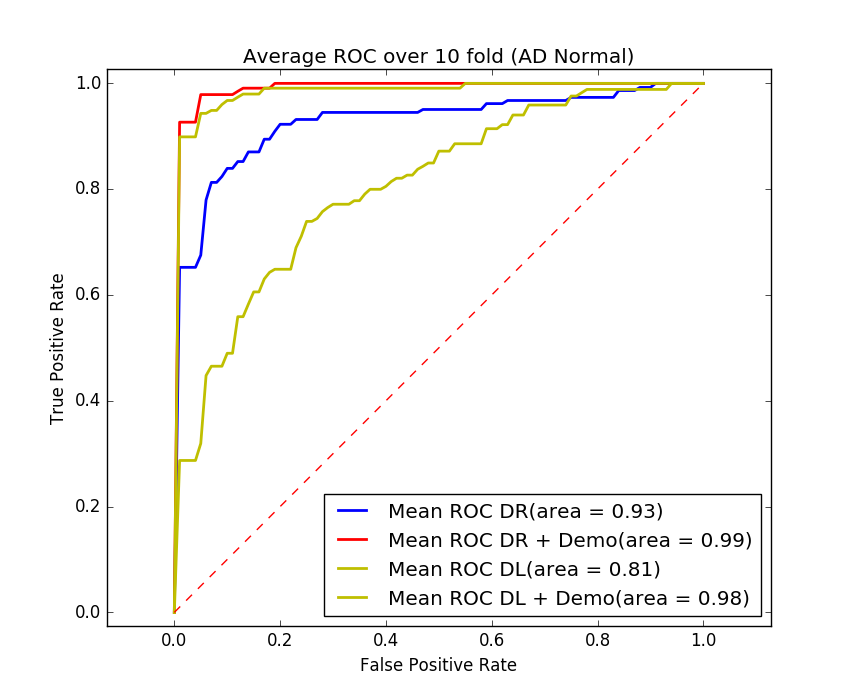
\includegraphics[width=\linewidth]{figures/AD_CU}
	\caption[ROC for AD vs. CU]{Classification in AD vs. CU group with different features performance comparison with receiver operating characteristic (ROC) curves and area under curve (AUC) measures. The results for DR and DR + Demographic are computed with the proposed method in Alg.\ref{alg:pipeline1}and DL and DL + Demographic are computed with the proposed method in Alg.\ref{alg:pipeline2}. Within the four statistics, the result of using Feature Extraction with Voxles, APOE and FAQ are better than others. Among all AUC measures, DR+Demo feature achieved the best performance (AUC = 0.99).}
	\label{fig:adcu}
\end{figure}
\begin{figure}[h]
	\centering
	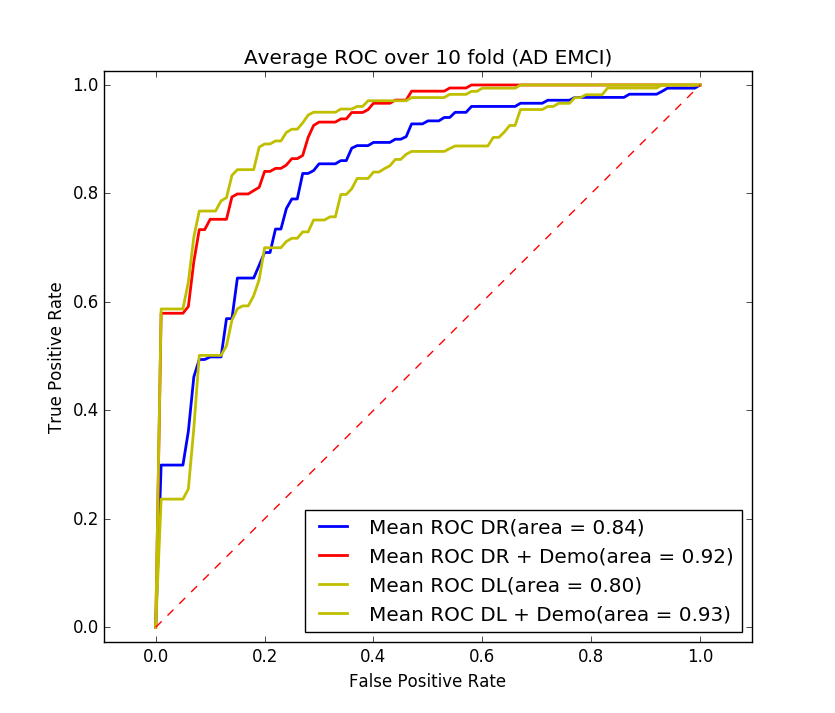
\includegraphics[width=\linewidth]{figures/AD_EMCI}
	\caption[ROC for AD vs. EMCI]{Classification in AD vs. CU group with different features performance comparison with receiver operating characteristic (ROC) curves and area under curve (AUC) measures. The results for DR and DR + Demographic are computed with the proposed method in Alg.\ref{alg:pipeline1}and DL and DL + Demographic are computed with the proposed method in Alg.\ref{alg:pipeline2}. Within the four statistics, the result of using Dictionary Learning with Voxles, APOE and FAQ are better than others.  Among all AUC measures, DL+Demo feature achieved the best performance (AUC = 0.93).}
	\label{fig:ademci}
\end{figure}
\begin{figure}[h]
	\centering
	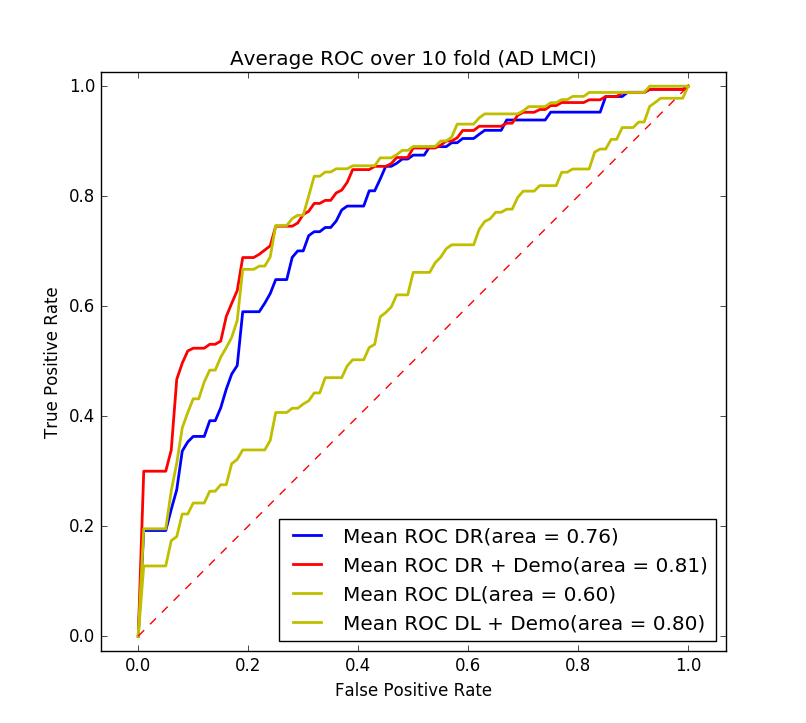
\includegraphics[width=\linewidth]{figures/AD_LMCI}
	\caption[ROC for AD vs. LMCI]{Classification in AD vs. CU group with different features performance comparison with receiver operating characteristic (ROC) curves and area under curve (AUC) measures. The results for DR and DR + Demographic are computed with the proposed method in Alg.\ref{alg:pipeline1}and DL and DL + Demographic are computed with the proposed method in Alg.\ref{alg:pipeline2}. Within the four statistics, the result of using Feature Extraction with Voxles, APOE and FAQ are better than others. Among all AUC measures, DR+Demo feature achieved the best performance (AUC = 0.81).}
	\label{fig:adlmci}
\end{figure}
\begin{figure}[h]
	\centering
	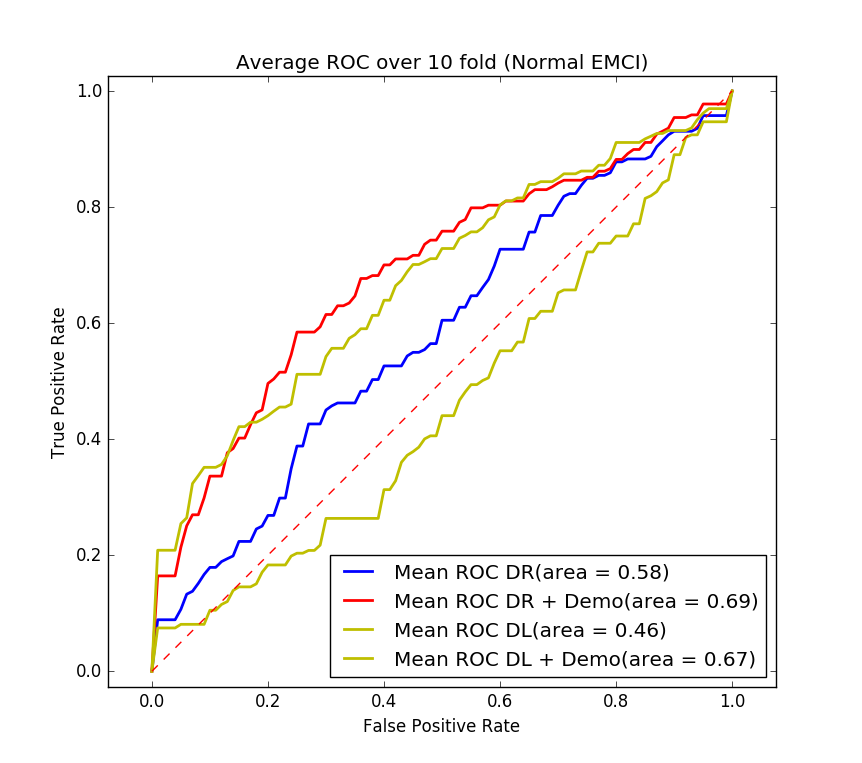
\includegraphics[width=\linewidth]{figures/CU_EMCI}
	\caption[ROC for Normal vs. EMCI]{Classification in AD vs. CU group with different features performance comparison with receiver operating characteristic (ROC) curves and area under curve (AUC) measures. The results for DR and DR + Demographic are computed with the proposed method in Alg.\ref{alg:pipeline1}and DL and DL + Demographic are computed with the proposed method in Alg.\ref{alg:pipeline2}. Within the four statistics, the result of using Feature Extraction with Voxles, APOE and FAQ are better than others. Among all AUC measures, DR+Demo feature achieved the best performance (AUC = 0.69).}
	\label{fig:cuemci}
\end{figure}
\begin{figure}[h]
	\centering
	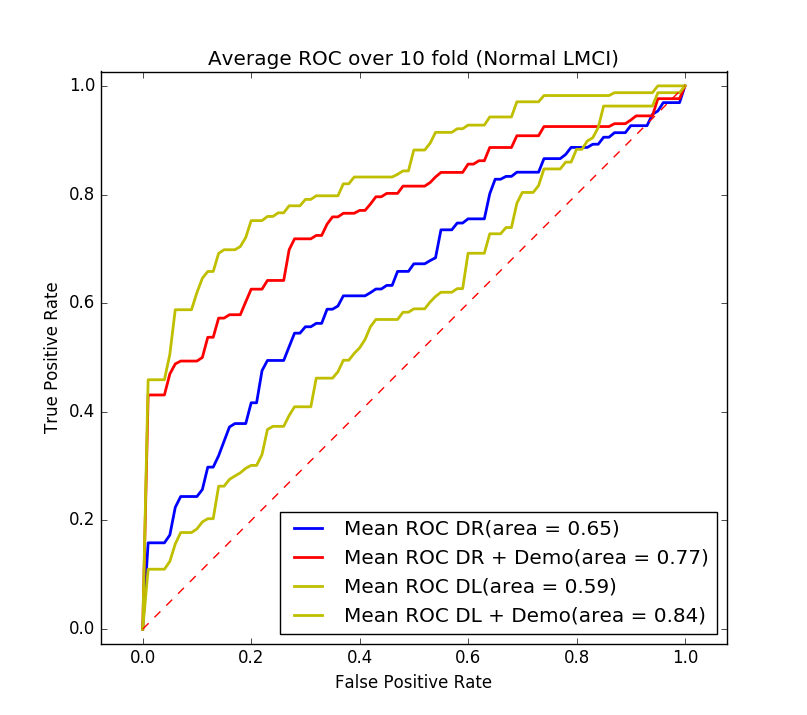
\includegraphics[width=\linewidth]{figures/CU_LMCI}
	\caption[ROC for Normal vs. LMCI]{Classification in AD vs. CU group with different features performance comparison with receiver operating characteristic (ROC) curves and area under curve (AUC) measures. The results for DR and DR + Demographic are computed with the proposed method in Alg.\ref{alg:pipeline1}and DL and DL + Demographic are computed with the proposed method in Alg.\ref{alg:pipeline2}. Within the four statistics, the result of using Dictionary Learning with Voxles, APOE and FAQ are better than others.  Among all AUC measures, DL+Demo feature achieved the best performance (AUC = 0.84).}
	\label{fig:culmci}
\end{figure}
\begin{figure}[h]
	\centering
	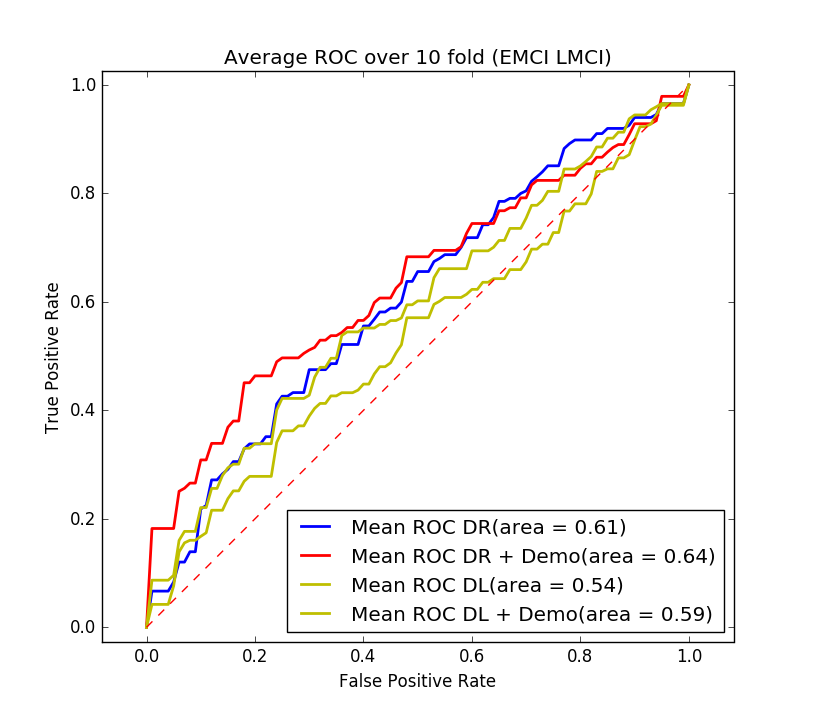
\includegraphics[width=\linewidth]{figures/EMCI_LMCI}
	\caption[ROC for EMCI vs. LMCI.]{Classification in AD vs. CU group with different features performance comparison with receiver operating characteristic (ROC) curves and area under curve (AUC) measures. The results for DR and DR + Demographic are computed with the proposed method in Alg.\ref{alg:pipeline1}and DL and DL + Demographic are computed with the proposed method in Alg.\ref{alg:pipeline2}. Within the four statistics, the result of using Feature Extraction with Voxles, APOE and FAQ are better than others. Among all AUC measures, DR+Demo feature achieved the best performance (AUC = 0.64).}
	\label{fig:emcilmci}
\end{figure}
